% Options for packages loaded elsewhere
\PassOptionsToPackage{unicode}{hyperref}
\PassOptionsToPackage{hyphens}{url}
\PassOptionsToPackage{dvipsnames,svgnames,x11names}{xcolor}
%
\documentclass[
  12pt,
]{article}
\usepackage{amsmath,amssymb}
\usepackage{lmodern}
\usepackage{iftex}
\ifPDFTeX
  \usepackage[T1]{fontenc}
  \usepackage[utf8]{inputenc}
  \usepackage{textcomp} % provide euro and other symbols
\else % if luatex or xetex
  \usepackage{unicode-math}
  \defaultfontfeatures{Scale=MatchLowercase}
  \defaultfontfeatures[\rmfamily]{Ligatures=TeX,Scale=1}
  \setmainfont[]{Times New Roman}
\fi
% Use upquote if available, for straight quotes in verbatim environments
\IfFileExists{upquote.sty}{\usepackage{upquote}}{}
\IfFileExists{microtype.sty}{% use microtype if available
  \usepackage[]{microtype}
  \UseMicrotypeSet[protrusion]{basicmath} % disable protrusion for tt fonts
}{}
\usepackage{xcolor}
\IfFileExists{xurl.sty}{\usepackage{xurl}}{} % add URL line breaks if available
\IfFileExists{bookmark.sty}{\usepackage{bookmark}}{\usepackage{hyperref}}
\hypersetup{
  pdftitle={Policy Effects on Mixed-Citizenship, Same-Sex Couples: A Triple-Difference Analysis},
  pdfauthor={Nathan I. Hoffmann, Department of Sociology, University of California, Los Angeles; Kristopher Velasco, Department of Sociology, Princeton University},
  colorlinks=true,
  linkcolor={blue},
  filecolor={Maroon},
  citecolor={Blue},
  urlcolor={Blue},
  pdfcreator={LaTeX via pandoc}}
\urlstyle{same} % disable monospaced font for URLs
\usepackage[margin=1in]{geometry}
\usepackage{longtable,booktabs,array}
\usepackage{calc} % for calculating minipage widths
% Correct order of tables after \paragraph or \subparagraph
\usepackage{etoolbox}
\makeatletter
\patchcmd\longtable{\par}{\if@noskipsec\mbox{}\fi\par}{}{}
\makeatother
% Allow footnotes in longtable head/foot
\IfFileExists{footnotehyper.sty}{\usepackage{footnotehyper}}{\usepackage{footnote}}
\makesavenoteenv{longtable}
\usepackage{graphicx}
\makeatletter
\def\maxwidth{\ifdim\Gin@nat@width>\linewidth\linewidth\else\Gin@nat@width\fi}
\def\maxheight{\ifdim\Gin@nat@height>\textheight\textheight\else\Gin@nat@height\fi}
\makeatother
% Scale images if necessary, so that they will not overflow the page
% margins by default, and it is still possible to overwrite the defaults
% using explicit options in \includegraphics[width, height, ...]{}
\setkeys{Gin}{width=\maxwidth,height=\maxheight,keepaspectratio}
% Set default figure placement to htbp
\makeatletter
\def\fps@figure{htbp}
\makeatother
\setlength{\emergencystretch}{3em} % prevent overfull lines
\providecommand{\tightlist}{%
  \setlength{\itemsep}{0pt}\setlength{\parskip}{0pt}}
\setcounter{secnumdepth}{5}
\newlength{\cslhangindent}
\setlength{\cslhangindent}{1.5em}
\newlength{\csllabelwidth}
\setlength{\csllabelwidth}{3em}
\newlength{\cslentryspacingunit} % times entry-spacing
\setlength{\cslentryspacingunit}{\parskip}
\newenvironment{CSLReferences}[2] % #1 hanging-ident, #2 entry spacing
 {% don't indent paragraphs
  \setlength{\parindent}{0pt}
  % turn on hanging indent if param 1 is 1
  \ifodd #1
  \let\oldpar\par
  \def\par{\hangindent=\cslhangindent\oldpar}
  \fi
  % set entry spacing
  \setlength{\parskip}{#2\cslentryspacingunit}
 }%
 {}
\usepackage{calc}
\newcommand{\CSLBlock}[1]{#1\hfill\break}
\newcommand{\CSLLeftMargin}[1]{\parbox[t]{\csllabelwidth}{#1}}
\newcommand{\CSLRightInline}[1]{\parbox[t]{\linewidth - \csllabelwidth}{#1}\break}
\newcommand{\CSLIndent}[1]{\hspace{\cslhangindent}#1}
\usepackage{setspace}\doublespace
\usepackage{bbm}
\usepackage{booktabs}
\usepackage{longtable}
\usepackage{array}
\usepackage{multirow}
\usepackage{wrapfig}
\usepackage{float}
\usepackage{colortbl}
\usepackage{pdflscape}
\usepackage{tabu}
\usepackage{threeparttable}
\usepackage{threeparttablex}
\usepackage[normalem]{ulem}
\usepackage{makecell}
\usepackage{xcolor}
\usepackage{caption}
\usepackage{graphicx}
\usepackage{siunitx}
\usepackage{hhline}
\usepackage{calc}
\usepackage{tabularx}
\usepackage{adjustbox}
\usepackage{hyperref}
\ifLuaTeX
  \usepackage{selnolig}  % disable illegal ligatures
\fi

\title{Policy Effects on Mixed-Citizenship, Same-Sex Couples: A Triple-Difference Analysis}
\author{Nathan I. Hoffmann, Department of Sociology, University of California, Los Angeles \and Kristopher Velasco, Department of Sociology, Princeton University}
\date{June 22, 2022}

\begin{document}
\maketitle
\begin{abstract}
After the U.S. Supreme Court struck down the Defense of Marriage Act (DOMA) in 2013, same-sex partners of U.S. citizens became eligible for spousal visas. Since then, the U.S. has a seen a rapid rise in same-sex, mixed-citizenship couples. However, this effect varies greatly depending on the LGB policy context of the non-citizen's country of origin. Using waves 2008 to 2019 of the American Community Survey, this study employs a triple-difference design to examine how the policy environment of the origin country moderates the effect of the end of DOMA. Quasi-Poisson models with two-way fixed effects show that, after 2013, individuals in mixed-citizenship same-sex couples coming from countries with progressive LGB policy saw a more than 50-percent increase in incidence relative to those in different-sex or same-citizenship couples. Meanwhile, those from countries with repressive laws experienced no relative increase. We argue that the policy context of country of origin leaves a lasting cultural impact on immigrants that shapes their response to policy shifts in their country of residence, even many years after migration.
\end{abstract}

\hypertarget{introduction}{%
\section{Introduction}\label{introduction}}

The policy environment for lesbian, gay, and bisexual (LGB) couples around the world has changed rapidly in recent years. In many countries, previously unthinkable rights to same-sex sexual relations, marriage, and employment security have become the law of the land. At the same time, retrenchment in other countries have resulted in increasingly repressive policies for LGB individuals (\protect\hyperlink{ref-gevisser_2020_pink}{Gevisser 2020}; \protect\hyperlink{ref-velasco_2022_opposition}{Velasco 2022}). Such policy shifts have wide-ranging effects not only on residents of those countries, but on LGB migrants who move between them (\protect\hyperlink{ref-ahmad_2013}{Ahmad 2013}; \protect\hyperlink{ref-carrillo_2018}{Carrillo 2018}; \protect\hyperlink{ref-mai_2009}{Mai and King 2009}; \protect\hyperlink{ref-gorman-murray_2009}{Gorman-Murray 2009}; \protect\hyperlink{ref-vogler_2016}{Vogler 2016}).

One policy change especially relevant to immigrants is the 2013 U.S. Supreme Court decision ruling the Defense of Marriage Act (DOMA) unconstitutional. For the first time, U.S. citizens could sponsor the visa of their same-sex spouse (\protect\hyperlink{ref-edwards_2013}{Edwards 2013}). In the years since, the U.S. population of immigrant-containing same-sex couples has grown rapidly (\protect\hyperlink{ref-hoffmann_2021_making}{Hoffmann and Velasco 2021}; \protect\hyperlink{ref-redpath_2022_spousal}{Redpath 2022}). Data on cohabiting partners and spouses from the American Community Survey (ACS, \protect\hyperlink{ref-ruggles_2021}{Ruggles et al. 2021}) shows that numbers of different-sex, mixed-citizenship couples grew by 8 percent from 2013 to 2019 (from 4.2 million to 4.5 million), while corresponding same-sex couples grew from 38 thousand to 96 thousand in the same period, an increase of 156 percent.

How can we understand the rapid rise of this type of union? Are trends homogeneous across the population of mixed-citizenship same-sex couples? As shown in Figure \ref{fig:desc}, this rapid increase after 2013 was not uniform across immigrants from all countries. For those hailing from countries with progressive LGB policies, the increase was indeed rapid after 2013. However, from those with repressive LGB policies, no increase occurred. Why do we so so much variation by policy context at the country of origin?

\begin{figure}
\centering
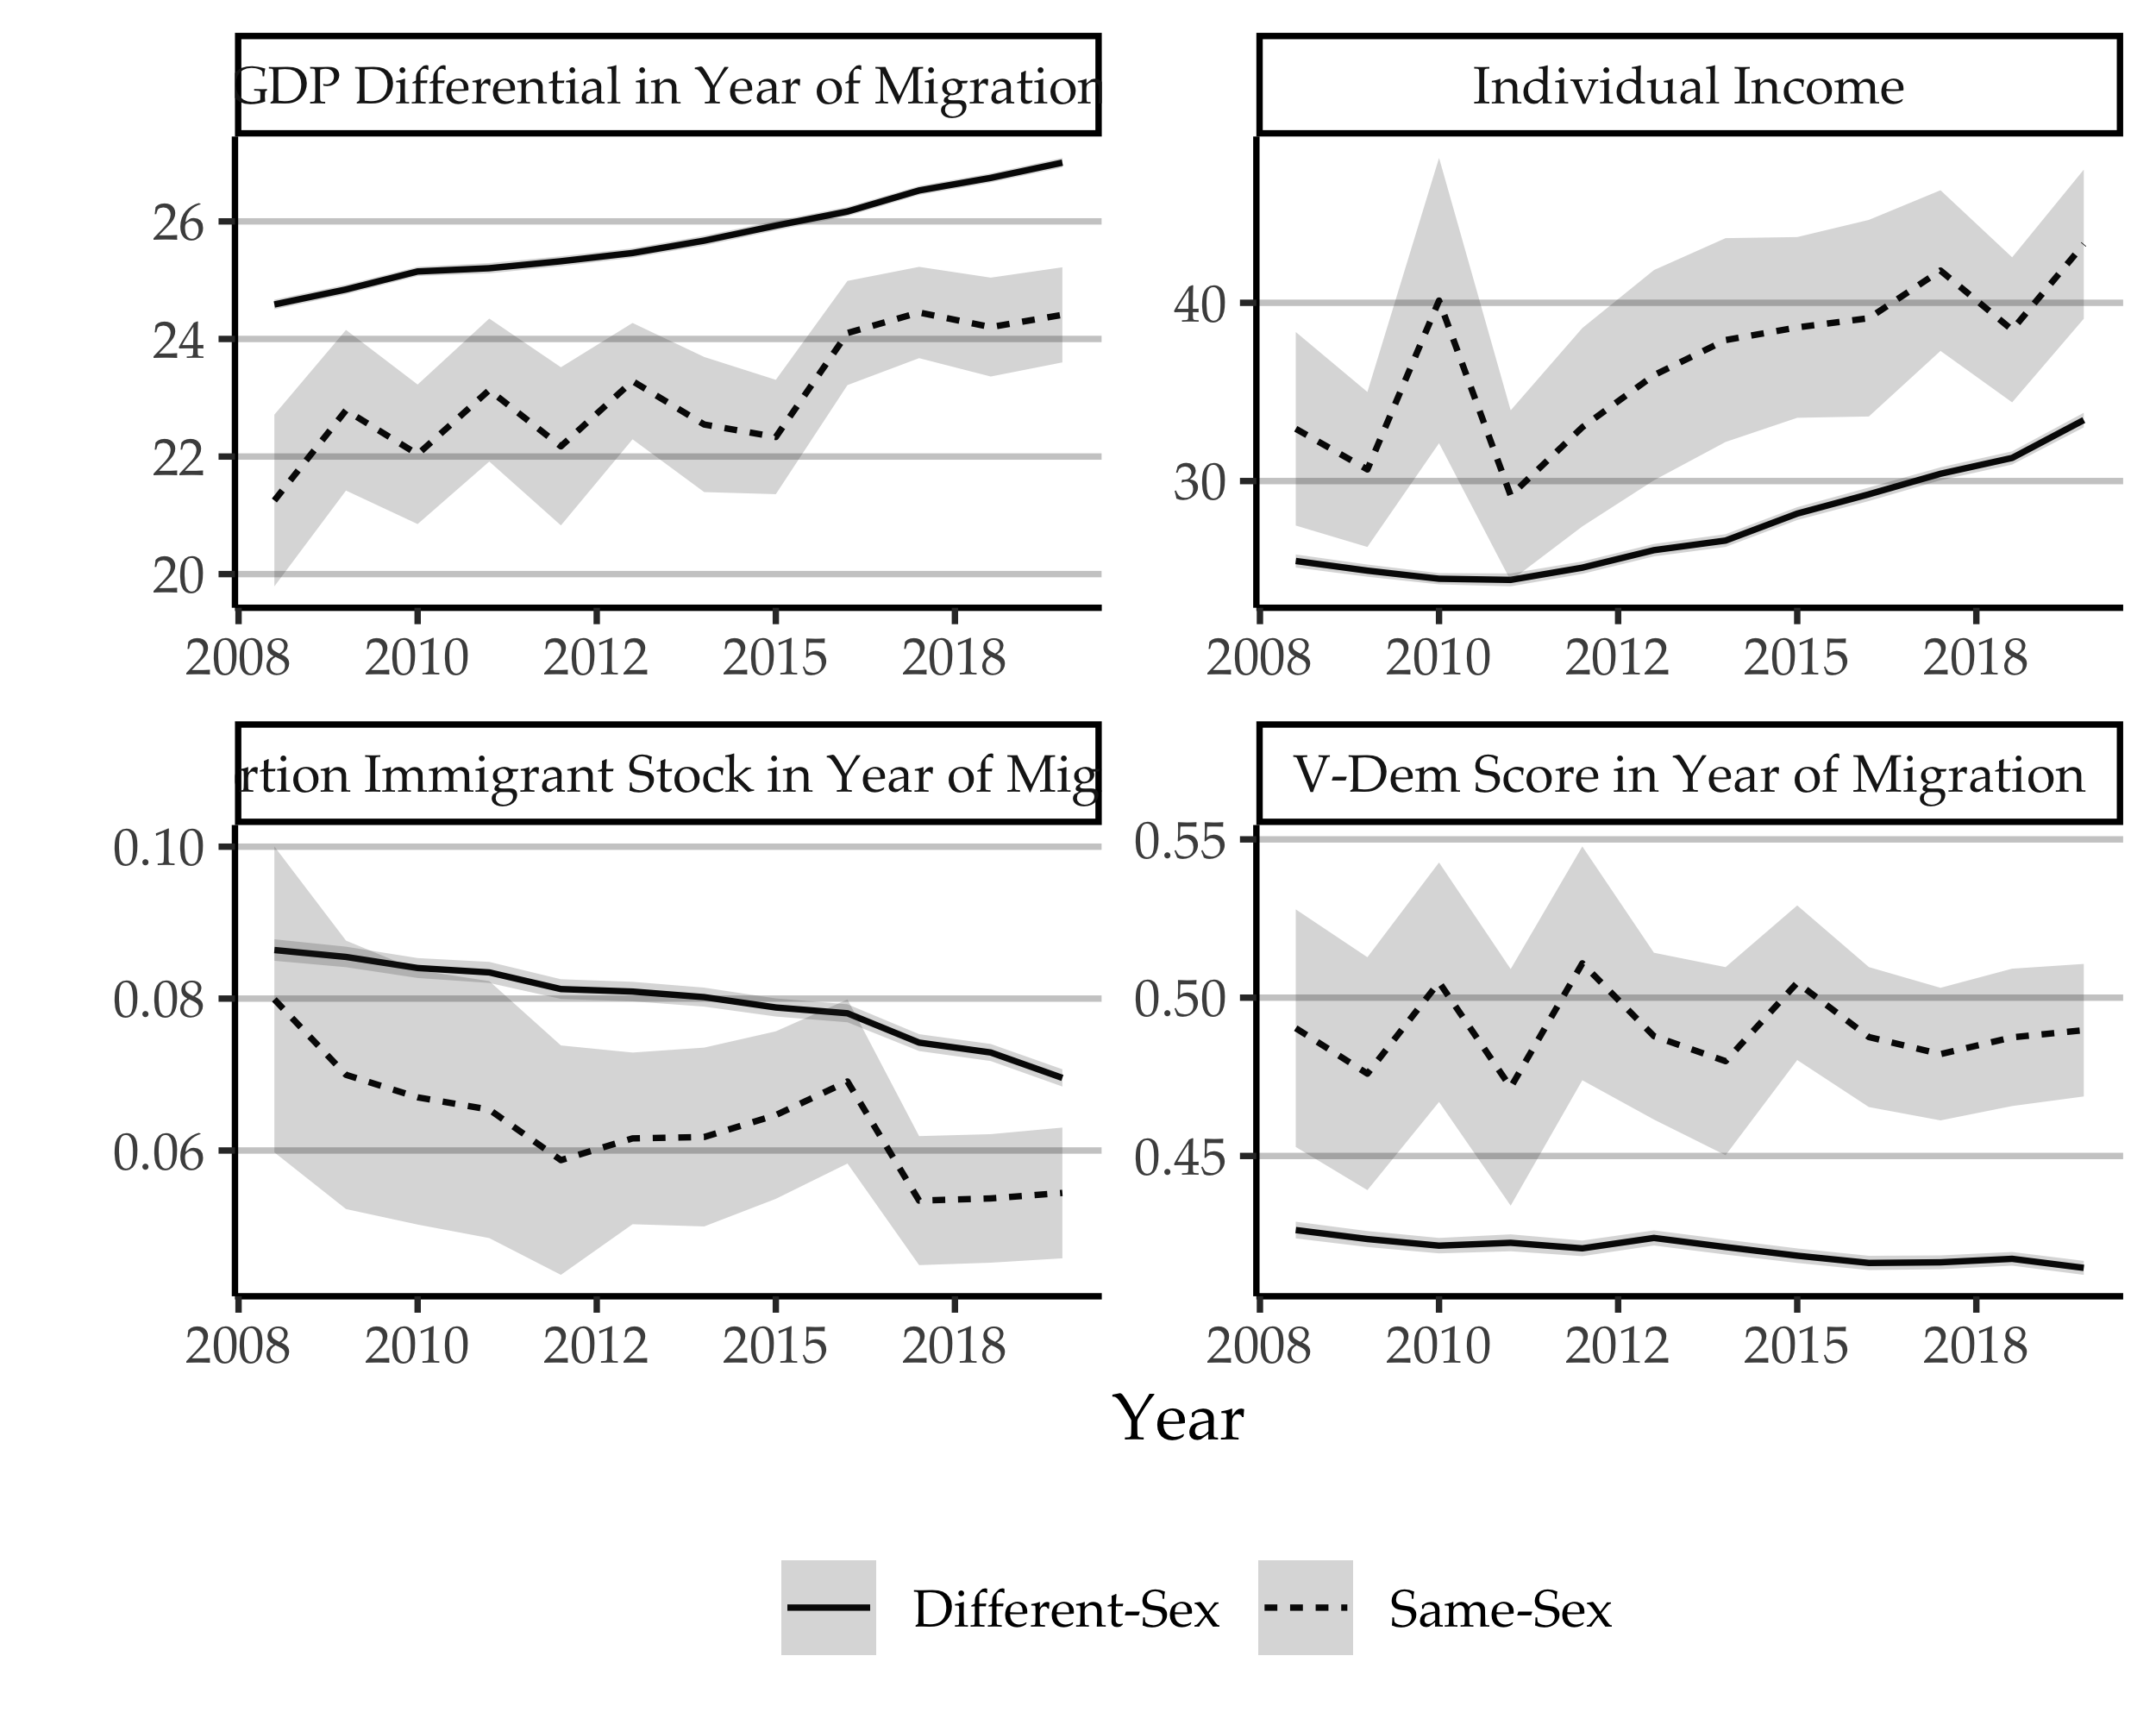
\includegraphics{ssimm_did_files/figure-latex/desc-1.pdf}
\caption{\label{fig:desc}Estimated counts of individuals in mixed-citizenship, same-same couples from the American Community Survey. The ``Repressive'' sample includes only countries with a LGB policy score less than 0, and the ``Progressive'' sample includes only those with a score greater than 3.}
\end{figure}

We argue that, like all relationship forms, same-sex unions are a cultural form that is specific to time and place (\protect\hyperlink{ref-kalmijn_2007_explaining}{Kalmijn 2007}; \protect\hyperlink{ref-treas_2014_attitudes}{Treas, Lui, and Gubernskaya 2014}; \protect\hyperlink{ref-wang_2018_coming}{Wang and Schofer 2018}). By defining what is possible, state policy helps shape the cultural products to which individuals aspire. Same-sex unions were unthinkable for many until very recently; progressive LGB policy institutionalizes this new cultural form in a recursive process, as access to this right increases support for it, and vice versa (\protect\hyperlink{ref-baiocco_2014_desire}{Baiocco, Argalia, and Laghi 2014}). On the other hand, repressive LGB policy limits the horizon of union possibilities, instills fear of punishment for disclosing one's same-sex union, and may even influence whether U.S. immigration officials view same-sex relationships from these countries as credible (\protect\hyperlink{ref-carron_2015_marriagebased}{Carron 2015}). Hence, the DOMA repeal is more likely to function as a pathway to spousal visas when it aligns with the institutional context of an immigrant's country of origin.

To test our theory, we apply cutting-edge methods of causal inference. Using waves 2008 to 2019 of the ACS, we employ a triple difference, quasi-Poisson design to estimate the effect of the post-2013 legal context in the U.S. on numbers of mixed-citizenship same-sex couples reported in the ACS. By controlling for numbers of mixed-citizenship and same-citizenship couples that we would not expect to be impacted by this policy, this design allows us to isolate the effect of DOMA's repeal specifically on unions of interest (\protect\hyperlink{ref-redpath_2022_spousal}{Redpath 2022}). To assess the role of LGB policy at the country of origin, we rely on an original dataset indexing LGB policy changes in 123 countries from 1991 to 2019. We stratify the sample by the LGB policy context at the country of origin to examine how the policy environment of the origin country moderates the effect of the end of DOMA.

We find that, after 2013, individuals in mixed-citizenship same-sex couples hailing from countries with progressive LGB policy saw a more than 50-percent increase in incidence relative to those in different-sex or same-citizenship couples. Meanwhile, those from countries with repressive laws experienced no relative increase at all. This suggests that the policy context of country of origin leaves a lasting cultural impact on immigrants that shapes their response to policy shifts in their country of residence, even many years after migration.

Our work adds to and connects the burgeoning literature on the importance of culture in shaping both migration (\protect\hyperlink{ref-benson_2009}{Benson and O'Reilly 2009}; \protect\hyperlink{ref-dixon_2020}{Dixon 2020}; \protect\hyperlink{ref-thompson_2017_migration}{\textbf{thompson\_2017\_migration?}}) and union decisions (\protect\hyperlink{ref-wang_2018_coming}{Wang and Schofer 2018}; \protect\hyperlink{ref-msibi_2013_denied}{Msibi 2013}). By linking these fields, we show institutional forms may be relevant outside of their obvious domain of influence.

\hypertarget{background}{%
\section{Background}\label{background}}

\hypertarget{policy-context}{%
\subsection{Policy Context}\label{policy-context}}

The United States Supreme Court overturned the Defense of Marriage Act (DOMA) in United States v. Windsor in 2013. Enacted in 1996, DOMA banned the federal government from recognizing same-sex marriages. Even if same-sex marriages were legalized at the state level, then, such recognition did not unlock access to federal marriage benefits. Thus, the Windsor decision carried significant implications for same-sex couples as they could now jointly file federal tax returns, secure Social Security benefits, and participate in numerous other federal programs like the Supplemental Nutrition Assistance Program.

Another important consequence of the DOMA ruling was unlocking spousal visas for same-sex couples. The federal government has long provided a pathway for U.S. citizens to secure permanent residency, and eventual citizenship, for their migrant spouses and fiancés. But DOMA prevented access to these visas because the federal government did not recognize same-sex unions as legitimate or valid -- thus categorically denying access. Additionally, DOMA had a downstream effect where even if a U.S. state were to legalize marriage, mixed-citizenship couples (where one partner is a U.S. citizen and where the other is a non-citizen) were unlikely to take advantage of these state-level benefits. This is because a condition of non-permanent residents' visas is to not show intent on staying in the U.S. permanently -- something marriage to a U.S. citizen can potentially violate. The Windsor decision allowed mixed-citizenship couples access to spousal visas and, where legal, for such couples to get married and switch visa types. As a direct consequence of undoing DOMA, Redpath (\protect\hyperlink{ref-redpath_2022_spousal}{2022}) finds a 36 percent relative increase in partnering of mixed-citizenship same-sex couples and a 78 percent increase in these types of marriages.

These increases in mixed-citizen couplings as found by Redpath are significant. The dramatic rise in mixed-citizen couplings can be the result of two distinct mechanisms: An increased entry into such unions of individuals already residing in the U.S. and the direct immigration of one or both members of the couple into the U.S. due to the policy shift. Regardless of pathway, these rising trends open new questions, such as: What are the characteristics of immigrants selecting into these relationships?

\hypertarget{country-of-origin-and-selection-into-same-sex-unions}{%
\subsection{Country of Origin and Selection into Same-Sex Unions}\label{country-of-origin-and-selection-into-same-sex-unions}}

Although the DOMA decision equally applied to all mixed-citizenship couples, Figure \ref{fig:desc} highlights an important line of differentiation: There is a distinct rise in couples where the non-U.S. citizen came from a country with more progressive LGB policies. Numbers of couples where the non-U.S. citizen came from a country with repressive LGB policies, such as bans on sodomy, remain unchanged. Why might this be? Why would conditions at the immigrant partner's country of origin influence the distribution of same-sex union formation across the population of mixed-citizen couples within the U.S.? We argue that by investigating the interplay between law and culture, we can understand the diverging trends found in Figure \ref{fig:desc}.

Relationships, and marriage specifically, are unique cultural products (\protect\hyperlink{ref-rosenfeld_2007_age}{Rosenfeld 2007}). The rituals, symbols, norms, and roles that govern them have different instantiations depending on the time and place. These cultural products then influence and are influenced by the legal expectations and conditions associated with relationships (\protect\hyperlink{ref-kalmijn_2007_explaining}{Kalmijn 2007}; \protect\hyperlink{ref-treas_2014_attitudes}{Treas, Lui, and Gubernskaya 2014}; \protect\hyperlink{ref-wang_2018_coming}{Wang and Schofer 2018}). This is especially true for same-sex unions in the present historical moment (\protect\hyperlink{ref-hull_2003_cultural}{Hull 2003}; \protect\hyperlink{ref-ocobock_2020_leveraging}{Ocobock 2020}). The assimilation of same-sex couples into existing marriage and relationship programs is a very current, dynamic process
(\protect\hyperlink{ref-bernstein_2013_marrying}{Bernstein and Taylor 2013}; \protect\hyperlink{ref-saez_2011_samesex}{Saez 2011}). Denmark became the first country to recognize civil unions for same-sex partners in 1989 while Netherlands became the first to grant full marriage equality in 2001. At the end of 2021, 31 countries had recognized full marriage equality with an additional 13 recognizing civil unions.

Of the many consequences of these shifts toward more progressive policies, one is that they shift our understanding of what it permissible and seen as possible. Prior to state recognition, there are often public campaigns by LGBT+ organizers seeking to influence broad support. While geared toward the general public, this campaign rhetoric and imagery also socializes LGB individuals into the appropriateness of participating in institutions long exclusive to heterosexuals (\protect\hyperlink{ref-bernstein_2013_marrying}{Bernstein and Taylor 2013}). This is particularly important as participation in same-sex unions by LGB individuals is a critical strategy to normalize and secure such legal advancements (\protect\hyperlink{ref-ocobock_2020_leveraging}{Ocobock 2020}). State recognition of same-sex couples also takes on a recursive process of increasing desirability of forming such a union as participation becomes a real option (\protect\hyperlink{ref-baiocco_2014_desire}{Baiocco, Argalia, and Laghi 2014}). Thus, immigrants coming from a country with an affirming policy environment that recognizes the validity of same-sex unions may be more inclined to establish and desire such a union once permitted to do so following DOMA.

Conversely, policy environments that are especially repressive can hinder the formation of mixed-citizenship, same-sex unions by immigrants in the U.S. This can operate in multiple ways. First, repressive contexts can potentially limit the desirability of forming a same-sex union by limiting what is seen as possible. At the end of 2021, roughly 70 countries still criminalized same-sex sexual acts between two consenting adults {[}xx{]}. While in some countries these laws are rarely enforced, in others, such as Cameroon, there has been an active revival of these laws to terrorize LGB populations (\protect\hyperlink{ref-bongmba_2021_samesex}{Bongmba 2021}). Moreover, the DOMA legislation in the U.S. was not a unique act. More than 30 countries since the 1990s have similarly re-codified a ``one man, one woman'' definition of marriage either through federal law like DOMA or through constitutional amendments {[}xx{]}. Second, these legal environments can influence how the cultural norms, rituals, and performances of relationships manifest. In the U.S. and many Western countries where marriage equality exists, mainstream LGB cultures emphasize publicly ``coming out'' and sameness with heterosexuals using language such as ``love is love.'' But LGB cultures where ``coming out'' risks vulnerability state-sponsored violence can look quite different (\protect\hyperlink{ref-msibi_2013_denied}{Msibi 2013}). Third, and relatedly, these different cultures can negatively influence whether U.S. immigration bureaucrats in charge of issuing visas perceive relationships as legitimate (\protect\hyperlink{ref-carron_2015_marriagebased}{Carron 2015}). When photos, disclosure to friends and family, and other public pieces of evidence are used to evaluate if a relationship is valid and worthy of a visa, immigrants coming from countries where such pieces of evidence can be harmful are at a systematic disadvantage. Thus, for all of these reasons, mixed-citizen, same-sex unions following the 2013 DOMA decision are likely to contain fewer immigrant partners from repressive contexts.

\hypertarget{data-and-methods}{%
\section{Data and Methods}\label{data-and-methods}}

\hypertarget{data}{%
\subsection{Data}\label{data}}

We employ data from the 2008 to 2019 American Community Survey (\protect\hyperlink{ref-ruggles_2021}{Ruggles et al. 2021}). Each year, the ACS surveys a 1-percent representative sample of the U.S. population about a variety of individual and household attributes. We focus on counts of individuals in mixed-citizenship same-sex couples, comparing to those in same-citizenship or different-sex couples. Our counts include only cohabiting individuals who identify themselves as spouses or unmarried partners, since the ACS does not allow identification of same-sex couples that do not reside together. ``Mixed-citizenship'' couples include either two citizens or two non-citizens, and ``same-sex'' couples include two individuals who report the same sex. We exclude individuals who immigrated before the age of 18 as well as those younger than 18 or older than 64 in each survey year.

Beginning in 2008 the Census Bureau made changes to ACS gender and partnership questions in order to prevent such errors (\protect\hyperlink{ref-u.s.censusbureau_2013}{U.S. Census Bureau 2013}), so we rely on data only from 2008 onward. In addition, following Gates and Steinberger (\protect\hyperlink{ref-gates_2009}{2009}), we remove all respondents that had either their relationship or sex variable imputed by the Census Bureau. See Table \ref{tab:data-tab} for sample sizes.

\providecommand{\docline}[3]{\noalign{\global\setlength{\arrayrulewidth}{#1}}\arrayrulecolor[HTML]{#2}\cline{#3}}

\setlength{\tabcolsep}{2pt}

\renewcommand*{\arraystretch}{1.5}

\begin{longtable}[c]{|p{1.09in}|p{1.38in}|p{1.21in}|p{1.16in}}

\caption{Unweighted and weighted sample sizes from American Community Survey (ACS) data, 2008-2019}\label{tab:data-tab}\\

\hhline{>{\arrayrulecolor[HTML]{666666}\global\arrayrulewidth=2pt}->{\arrayrulecolor[HTML]{666666}\global\arrayrulewidth=2pt}->{\arrayrulecolor[HTML]{666666}\global\arrayrulewidth=2pt}->{\arrayrulecolor[HTML]{666666}\global\arrayrulewidth=2pt}-}

\multicolumn{1}{!{\color[HTML]{000000}\vrule width 0pt}>{\raggedright}p{\dimexpr 1.09in+0\tabcolsep+0\arrayrulewidth}}{\fontsize{11}{11}\selectfont{\textcolor[HTML]{000000}{\global\setmainfont{Times New Roman}{Composition}}}} & \multicolumn{1}{!{\color[HTML]{000000}\vrule width 0pt}>{\raggedright}p{\dimexpr 1.38in+0\tabcolsep+0\arrayrulewidth}}{\fontsize{11}{11}\selectfont{\textcolor[HTML]{000000}{\global\setmainfont{Times New Roman}{Citizenship}}}} & \multicolumn{1}{!{\color[HTML]{000000}\vrule width 0pt}>{\raggedleft}p{\dimexpr 1.21in+0\tabcolsep+0\arrayrulewidth}}{\fontsize{11}{11}\selectfont{\textcolor[HTML]{000000}{\global\setmainfont{Times New Roman}{n\ (unweighted)}}}} & \multicolumn{1}{!{\color[HTML]{000000}\vrule width 0pt}>{\raggedleft}p{\dimexpr 1.16in+0\tabcolsep+0\arrayrulewidth}!{\color[HTML]{000000}\vrule width 0pt}}{\fontsize{11}{11}\selectfont{\textcolor[HTML]{000000}{\global\setmainfont{Times New Roman}{n\ (weighted)}}}} \\

\noalign{\global\setlength{\arrayrulewidth}{2pt}}\arrayrulecolor[HTML]{666666}\cline{1-4}

\endfirsthead

\hhline{>{\arrayrulecolor[HTML]{666666}\global\arrayrulewidth=2pt}->{\arrayrulecolor[HTML]{666666}\global\arrayrulewidth=2pt}->{\arrayrulecolor[HTML]{666666}\global\arrayrulewidth=2pt}->{\arrayrulecolor[HTML]{666666}\global\arrayrulewidth=2pt}-}

\multicolumn{1}{!{\color[HTML]{000000}\vrule width 0pt}>{\raggedright}p{\dimexpr 1.09in+0\tabcolsep+0\arrayrulewidth}}{\fontsize{11}{11}\selectfont{\textcolor[HTML]{000000}{\global\setmainfont{Times New Roman}{Composition}}}} & \multicolumn{1}{!{\color[HTML]{000000}\vrule width 0pt}>{\raggedright}p{\dimexpr 1.38in+0\tabcolsep+0\arrayrulewidth}}{\fontsize{11}{11}\selectfont{\textcolor[HTML]{000000}{\global\setmainfont{Times New Roman}{Citizenship}}}} & \multicolumn{1}{!{\color[HTML]{000000}\vrule width 0pt}>{\raggedleft}p{\dimexpr 1.21in+0\tabcolsep+0\arrayrulewidth}}{\fontsize{11}{11}\selectfont{\textcolor[HTML]{000000}{\global\setmainfont{Times New Roman}{n\ (unweighted)}}}} & \multicolumn{1}{!{\color[HTML]{000000}\vrule width 0pt}>{\raggedleft}p{\dimexpr 1.16in+0\tabcolsep+0\arrayrulewidth}!{\color[HTML]{000000}\vrule width 0pt}}{\fontsize{11}{11}\selectfont{\textcolor[HTML]{000000}{\global\setmainfont{Times New Roman}{n\ (weighted)}}}} \\

\noalign{\global\setlength{\arrayrulewidth}{2pt}}\arrayrulecolor[HTML]{666666}\cline{1-4}\endhead



\multicolumn{1}{!{\color[HTML]{000000}\vrule width 0pt}>{\raggedright}p{\dimexpr 1.09in+0\tabcolsep+0\arrayrulewidth}}{\fontsize{11}{11}\selectfont{\textcolor[HTML]{000000}{\global\setmainfont{Times New Roman}{Different\ sex}}}} & \multicolumn{1}{!{\color[HTML]{000000}\vrule width 0pt}>{\raggedright}p{\dimexpr 1.38in+0\tabcolsep+0\arrayrulewidth}}{\fontsize{11}{11}\selectfont{\textcolor[HTML]{000000}{\global\setmainfont{Times New Roman}{Mixed\ citizenship}}}} & \multicolumn{1}{!{\color[HTML]{000000}\vrule width 0pt}>{\raggedleft}p{\dimexpr 1.21in+0\tabcolsep+0\arrayrulewidth}}{\fontsize{11}{11}\selectfont{\textcolor[HTML]{000000}{\global\setmainfont{Times New Roman}{467,611}}}} & \multicolumn{1}{!{\color[HTML]{000000}\vrule width 0pt}>{\raggedleft}p{\dimexpr 1.16in+0\tabcolsep+0\arrayrulewidth}!{\color[HTML]{000000}\vrule width 0pt}}{\fontsize{11}{11}\selectfont{\textcolor[HTML]{000000}{\global\setmainfont{Times New Roman}{50,313,621}}}} \\





\multicolumn{1}{!{\color[HTML]{000000}\vrule width 0pt}>{\raggedright}p{\dimexpr 1.09in+0\tabcolsep+0\arrayrulewidth}}{\fontsize{11}{11}\selectfont{\textcolor[HTML]{000000}{\global\setmainfont{Times New Roman}{Different\ sex}}}} & \multicolumn{1}{!{\color[HTML]{000000}\vrule width 0pt}>{\raggedright}p{\dimexpr 1.38in+0\tabcolsep+0\arrayrulewidth}}{\fontsize{11}{11}\selectfont{\textcolor[HTML]{000000}{\global\setmainfont{Times New Roman}{Same\ citizenship}}}} & \multicolumn{1}{!{\color[HTML]{000000}\vrule width 0pt}>{\raggedleft}p{\dimexpr 1.21in+0\tabcolsep+0\arrayrulewidth}}{\fontsize{11}{11}\selectfont{\textcolor[HTML]{000000}{\global\setmainfont{Times New Roman}{11,103,024}}}} & \multicolumn{1}{!{\color[HTML]{000000}\vrule width 0pt}>{\raggedleft}p{\dimexpr 1.16in+0\tabcolsep+0\arrayrulewidth}!{\color[HTML]{000000}\vrule width 0pt}}{\fontsize{11}{11}\selectfont{\textcolor[HTML]{000000}{\global\setmainfont{Times New Roman}{1,046,422,984}}}} \\





\multicolumn{1}{!{\color[HTML]{000000}\vrule width 0pt}>{\raggedright}p{\dimexpr 1.09in+0\tabcolsep+0\arrayrulewidth}}{\fontsize{11}{11}\selectfont{\textcolor[HTML]{000000}{\global\setmainfont{Times New Roman}{Same\ sex}}}} & \multicolumn{1}{!{\color[HTML]{000000}\vrule width 0pt}>{\raggedright}p{\dimexpr 1.38in+0\tabcolsep+0\arrayrulewidth}}{\fontsize{11}{11}\selectfont{\textcolor[HTML]{000000}{\global\setmainfont{Times New Roman}{Mixed\ citizenship}}}} & \multicolumn{1}{!{\color[HTML]{000000}\vrule width 0pt}>{\raggedleft}p{\dimexpr 1.21in+0\tabcolsep+0\arrayrulewidth}}{\fontsize{11}{11}\selectfont{\textcolor[HTML]{000000}{\global\setmainfont{Times New Roman}{7,305}}}} & \multicolumn{1}{!{\color[HTML]{000000}\vrule width 0pt}>{\raggedleft}p{\dimexpr 1.16in+0\tabcolsep+0\arrayrulewidth}!{\color[HTML]{000000}\vrule width 0pt}}{\fontsize{11}{11}\selectfont{\textcolor[HTML]{000000}{\global\setmainfont{Times New Roman}{694,122}}}} \\





\multicolumn{1}{!{\color[HTML]{000000}\vrule width 0pt}>{\raggedright}p{\dimexpr 1.09in+0\tabcolsep+0\arrayrulewidth}}{\fontsize{11}{11}\selectfont{\textcolor[HTML]{000000}{\global\setmainfont{Times New Roman}{Same\ sex}}}} & \multicolumn{1}{!{\color[HTML]{000000}\vrule width 0pt}>{\raggedright}p{\dimexpr 1.38in+0\tabcolsep+0\arrayrulewidth}}{\fontsize{11}{11}\selectfont{\textcolor[HTML]{000000}{\global\setmainfont{Times New Roman}{Same\ citizenship}}}} & \multicolumn{1}{!{\color[HTML]{000000}\vrule width 0pt}>{\raggedleft}p{\dimexpr 1.21in+0\tabcolsep+0\arrayrulewidth}}{\fontsize{11}{11}\selectfont{\textcolor[HTML]{000000}{\global\setmainfont{Times New Roman}{147,459}}}} & \multicolumn{1}{!{\color[HTML]{000000}\vrule width 0pt}>{\raggedleft}p{\dimexpr 1.16in+0\tabcolsep+0\arrayrulewidth}!{\color[HTML]{000000}\vrule width 0pt}}{\fontsize{11}{11}\selectfont{\textcolor[HTML]{000000}{\global\setmainfont{Times New Roman}{13,630,989}}}} \\

\noalign{\global\setlength{\arrayrulewidth}{2pt}}\arrayrulecolor[HTML]{666666}\cline{1-4}



\end{longtable}

Our analytic strategy proceeds in two parts. First, how does LGB policy at country of origin moderate the effect of the repeal of DOMA on the incidence of same-sex, mixed-citizenship couples in the U.S.? Second, which specific LGB policies of country of origin are most relevant in shaping entry into same-sex unions?

To isolate the effect of the 2013 DOMA repeal, we employ a triple difference, or difference-in-differences-in-differences (DDD), quasi-Poisson design (\protect\hyperlink{ref-hausman_1984_econometric}{Hausman, Hall, and Griliches 1984}; \protect\hyperlink{ref-olden_forthcoming_triple}{Olden and Møen forthcoming}). We model counts as draws from a Poisson distribution, but estimate our model more flexibly by using quasi-maximum likelihood estimation (QMLE). Unlike Maximum Likelihood Estimation (MLE), this estimation method does not assume the mean and variance of the distribution are equal, adjusting standard errors accordingly (\protect\hyperlink{ref-cameron_2005_microeconometrics}{Cameron and Trivedi 2005, 667}). We include two-way fixed effects, with indicators for survey year and state-group, and cluster standard errors at the state-group level.

Our estimand is the relative change in incidence of individual in mixed-citizenship, same-sex couples following the repeal of DOMA in 2013. We estimate this as the coefficient to a three-way interaction between indicators for same-sex, mixed-citizenship, and post-2013 survey year. We write our model as
\[\begin{aligned}
y_{gst} = &\exp(\beta_0 + \beta_1 post_t + \beta_2 M_g \times post_t + \beta_3 S_g \times post_t  \\
&+ \beta_4 M_g \times S_g \times post_g + \alpha_{gs} + \gamma_{t} + \epsilon_{gst})
\end{aligned}\]
where \(y_{gst}\) is the count of individuals in group \(g\) in state \(s\) in survey year \(t\); \(post_t\) is an indicator variable for \(t > 2013\); \(M_g\) is an indicator variable for group \(g\) being mixed-citizenship; \(S_g\) is an indicator variable for group \(g\) being same-sex; \(\alpha_{gs}\) are group-state fixed effects; \(\gamma_t\) are survey year fixed effects; and \(\epsilon_{gst}\) is an error term such that \(\mathbf E(\epsilon_{gst}) = 0\). The coefficient of interest is \(\beta_4\); the incidence ratio \(\exp(\beta_4)\) estimates the relative increase in mixed-citizenship same-sex couples after 2013, relative to other couples.

We focus on heterogeneity of this effect: how it varies by the LGB policy context of non-citizens' country of origin. We measure the origin country policy environment using a modified LGBT Policy Index (\protect\hyperlink{ref-velasco_2018}{Velasco 2018}) for 1991 to 2019. The index is created by summing the net total of progressive policies (scored \(+1\)) over regressive policies (scored \(-1\)). The country index ranges from -3 to 10, with a mean of 1.7 in our sample. Group-state-year-country cells are assigned the average score in the year of immigration for non-citizen individuals in that cell.

\hypertarget{results}{%
\section{Results}\label{results}}

 
  \providecommand{\huxb}[2]{\arrayrulecolor[RGB]{#1}\global\arrayrulewidth=#2pt}
  \providecommand{\huxvb}[2]{\color[RGB]{#1}\vrule width #2pt}
  \providecommand{\huxtpad}[1]{\rule{0pt}{#1}}
  \providecommand{\huxbpad}[1]{\rule[-#1]{0pt}{#1}}

\begin{table}[ht]
\begin{centerbox}
\begin{threeparttable}
\captionsetup{justification=centering,singlelinecheck=off}
\caption{\label{tab:mod-tab} Quasi-Poisson DDD regressions of counts of 
                        mixed-citizenship same-sex couples}
 \setlength{\tabcolsep}{0pt}
\begin{tabularx}{1\textwidth}{p{0.25\textwidth} p{0.25\textwidth} p{0.25\textwidth} p{0.25\textwidth}}


\hhline{>{\huxb{0, 0, 0}{0.8}}->{\huxb{0, 0, 0}{0.8}}->{\huxb{0, 0, 0}{0.8}}->{\huxb{0, 0, 0}{0.8}}-}
\arrayrulecolor{black}

\multicolumn{1}{!{\huxvb{0, 0, 0}{0}}p{0.25\textwidth}!{\huxvb{0, 0, 0}{0}}}{\hspace{0pt}\parbox[b]{0.25\textwidth-0pt-0pt}{\huxtpad{0pt + 1em}\centering \huxbpad{0pt}}} &
\multicolumn{1}{p{0.25\textwidth}!{\huxvb{0, 0, 0}{0}}}{\hspace{0pt}\parbox[b]{0.25\textwidth-0pt-0pt}{\huxtpad{0pt + 1em}\centering Full sample\huxbpad{0pt}}} &
\multicolumn{1}{p{0.25\textwidth}!{\huxvb{0, 0, 0}{0}}}{\hspace{0pt}\parbox[b]{0.25\textwidth-0pt-0pt}{\huxtpad{0pt + 1em}\centering Progressive\huxbpad{0pt}}} &
\multicolumn{1}{p{0.25\textwidth}!{\huxvb{0, 0, 0}{0}}}{\hspace{0pt}\parbox[b]{0.25\textwidth-0pt-0pt}{\huxtpad{0pt + 1em}\centering Repressive\huxbpad{0pt}}} \tabularnewline[-0.5pt]


\hhline{>{\huxb{255, 255, 255}{0.4}}->{\huxb{0, 0, 0}{0.4}}->{\huxb{0, 0, 0}{0.4}}->{\huxb{0, 0, 0}{0.4}}-}
\arrayrulecolor{black}

\multicolumn{1}{!{\huxvb{0, 0, 0}{0}}p{0.25\textwidth}!{\huxvb{0, 0, 0}{0}}}{\hspace{0pt}\parbox[b]{0.25\textwidth-0pt-0pt}{\huxtpad{0pt + 1em}\raggedright Post-2013 × Same-sex × Mixed-citizenship\huxbpad{0pt}}} &
\multicolumn{1}{p{0.25\textwidth}!{\huxvb{0, 0, 0}{0}}}{\hspace{0pt}\parbox[b]{0.25\textwidth-0pt-0pt}{\huxtpad{0pt + 1em}\raggedleft 0.326 ***\huxbpad{0pt}}} &
\multicolumn{1}{p{0.25\textwidth}!{\huxvb{0, 0, 0}{0}}}{\hspace{0pt}\parbox[b]{0.25\textwidth-0pt-0pt}{\huxtpad{0pt + 1em}\raggedleft 0.475 ***\huxbpad{0pt}}} &
\multicolumn{1}{p{0.25\textwidth}!{\huxvb{0, 0, 0}{0}}}{\hspace{0pt}\parbox[b]{0.25\textwidth-0pt-0pt}{\huxtpad{0pt + 1em}\raggedleft 0.103\hphantom{0}\hphantom{0}\hphantom{0}\hphantom{0}\huxbpad{0pt}}} \tabularnewline[-0.5pt]


\hhline{}
\arrayrulecolor{black}

\multicolumn{1}{!{\huxvb{0, 0, 0}{0}}p{0.25\textwidth}!{\huxvb{0, 0, 0}{0}}}{\hspace{0pt}\parbox[b]{0.25\textwidth-0pt-0pt}{\huxtpad{0pt + 1em}\raggedright \huxbpad{0pt}}} &
\multicolumn{1}{p{0.25\textwidth}!{\huxvb{0, 0, 0}{0}}}{\hspace{0pt}\parbox[b]{0.25\textwidth-0pt-0pt}{\huxtpad{0pt + 1em}\raggedleft (0.050)\hphantom{0}\hphantom{0}\hphantom{0}\huxbpad{0pt}}} &
\multicolumn{1}{p{0.25\textwidth}!{\huxvb{0, 0, 0}{0}}}{\hspace{0pt}\parbox[b]{0.25\textwidth-0pt-0pt}{\huxtpad{0pt + 1em}\raggedleft (0.100)\hphantom{0}\hphantom{0}\hphantom{0}\huxbpad{0pt}}} &
\multicolumn{1}{p{0.25\textwidth}!{\huxvb{0, 0, 0}{0}}}{\hspace{0pt}\parbox[b]{0.25\textwidth-0pt-0pt}{\huxtpad{0pt + 1em}\raggedleft (0.097)\hphantom{0}\hphantom{0}\hphantom{0}\huxbpad{0pt}}} \tabularnewline[-0.5pt]


\hhline{}
\arrayrulecolor{black}

\multicolumn{1}{!{\huxvb{0, 0, 0}{0}}p{0.25\textwidth}!{\huxvb{0, 0, 0}{0}}}{\hspace{0pt}\parbox[b]{0.25\textwidth-0pt-0pt}{\huxtpad{0pt + 1em}\raggedright Post-2013 × Same-sex\huxbpad{0pt}}} &
\multicolumn{1}{p{0.25\textwidth}!{\huxvb{0, 0, 0}{0}}}{\hspace{0pt}\parbox[b]{0.25\textwidth-0pt-0pt}{\huxtpad{0pt + 1em}\raggedleft 0.370 ***\huxbpad{0pt}}} &
\multicolumn{1}{p{0.25\textwidth}!{\huxvb{0, 0, 0}{0}}}{\hspace{0pt}\parbox[b]{0.25\textwidth-0pt-0pt}{\huxtpad{0pt + 1em}\raggedleft 0.373 ***\huxbpad{0pt}}} &
\multicolumn{1}{p{0.25\textwidth}!{\huxvb{0, 0, 0}{0}}}{\hspace{0pt}\parbox[b]{0.25\textwidth-0pt-0pt}{\huxtpad{0pt + 1em}\raggedleft 0.374 ***\huxbpad{0pt}}} \tabularnewline[-0.5pt]


\hhline{}
\arrayrulecolor{black}

\multicolumn{1}{!{\huxvb{0, 0, 0}{0}}p{0.25\textwidth}!{\huxvb{0, 0, 0}{0}}}{\hspace{0pt}\parbox[b]{0.25\textwidth-0pt-0pt}{\huxtpad{0pt + 1em}\raggedright \huxbpad{0pt}}} &
\multicolumn{1}{p{0.25\textwidth}!{\huxvb{0, 0, 0}{0}}}{\hspace{0pt}\parbox[b]{0.25\textwidth-0pt-0pt}{\huxtpad{0pt + 1em}\raggedleft (0.017)\hphantom{0}\hphantom{0}\hphantom{0}\huxbpad{0pt}}} &
\multicolumn{1}{p{0.25\textwidth}!{\huxvb{0, 0, 0}{0}}}{\hspace{0pt}\parbox[b]{0.25\textwidth-0pt-0pt}{\huxtpad{0pt + 1em}\raggedleft (0.018)\hphantom{0}\hphantom{0}\hphantom{0}\huxbpad{0pt}}} &
\multicolumn{1}{p{0.25\textwidth}!{\huxvb{0, 0, 0}{0}}}{\hspace{0pt}\parbox[b]{0.25\textwidth-0pt-0pt}{\huxtpad{0pt + 1em}\raggedleft (0.019)\hphantom{0}\hphantom{0}\hphantom{0}\huxbpad{0pt}}} \tabularnewline[-0.5pt]


\hhline{}
\arrayrulecolor{black}

\multicolumn{1}{!{\huxvb{0, 0, 0}{0}}p{0.25\textwidth}!{\huxvb{0, 0, 0}{0}}}{\hspace{0pt}\parbox[b]{0.25\textwidth-0pt-0pt}{\huxtpad{0pt + 1em}\raggedright Post-2013 × Mixed-citizenship\huxbpad{0pt}}} &
\multicolumn{1}{p{0.25\textwidth}!{\huxvb{0, 0, 0}{0}}}{\hspace{0pt}\parbox[b]{0.25\textwidth-0pt-0pt}{\huxtpad{0pt + 1em}\raggedleft 0.101 ***\huxbpad{0pt}}} &
\multicolumn{1}{p{0.25\textwidth}!{\huxvb{0, 0, 0}{0}}}{\hspace{0pt}\parbox[b]{0.25\textwidth-0pt-0pt}{\huxtpad{0pt + 1em}\raggedleft 0.283 ***\huxbpad{0pt}}} &
\multicolumn{1}{p{0.25\textwidth}!{\huxvb{0, 0, 0}{0}}}{\hspace{0pt}\parbox[b]{0.25\textwidth-0pt-0pt}{\huxtpad{0pt + 1em}\raggedleft 0.019\hphantom{0}\hphantom{0}\hphantom{0}\hphantom{0}\huxbpad{0pt}}} \tabularnewline[-0.5pt]


\hhline{}
\arrayrulecolor{black}

\multicolumn{1}{!{\huxvb{0, 0, 0}{0}}p{0.25\textwidth}!{\huxvb{0, 0, 0}{0}}}{\hspace{0pt}\parbox[b]{0.25\textwidth-0pt-0pt}{\huxtpad{0pt + 1em}\raggedright \huxbpad{0pt}}} &
\multicolumn{1}{p{0.25\textwidth}!{\huxvb{0, 0, 0}{0}}}{\hspace{0pt}\parbox[b]{0.25\textwidth-0pt-0pt}{\huxtpad{0pt + 1em}\raggedleft (0.015)\hphantom{0}\hphantom{0}\hphantom{0}\huxbpad{0pt}}} &
\multicolumn{1}{p{0.25\textwidth}!{\huxvb{0, 0, 0}{0}}}{\hspace{0pt}\parbox[b]{0.25\textwidth-0pt-0pt}{\huxtpad{0pt + 1em}\raggedleft (0.042)\hphantom{0}\hphantom{0}\hphantom{0}\huxbpad{0pt}}} &
\multicolumn{1}{p{0.25\textwidth}!{\huxvb{0, 0, 0}{0}}}{\hspace{0pt}\parbox[b]{0.25\textwidth-0pt-0pt}{\huxtpad{0pt + 1em}\raggedleft (0.049)\hphantom{0}\hphantom{0}\hphantom{0}\huxbpad{0pt}}} \tabularnewline[-0.5pt]


\hhline{}
\arrayrulecolor{black}

\multicolumn{1}{!{\huxvb{0, 0, 0}{0}}p{0.25\textwidth}!{\huxvb{0, 0, 0}{0}}}{\hspace{0pt}\parbox[b]{0.25\textwidth-0pt-0pt}{\huxtpad{0pt + 1em}\raggedright Post-2013\huxbpad{0pt}}} &
\multicolumn{1}{p{0.25\textwidth}!{\huxvb{0, 0, 0}{0}}}{\hspace{0pt}\parbox[b]{0.25\textwidth-0pt-0pt}{\huxtpad{0pt + 1em}\raggedleft -0.035 **\hphantom{0}\huxbpad{0pt}}} &
\multicolumn{1}{p{0.25\textwidth}!{\huxvb{0, 0, 0}{0}}}{\hspace{0pt}\parbox[b]{0.25\textwidth-0pt-0pt}{\huxtpad{0pt + 1em}\raggedleft -0.038 *\hphantom{0}\hphantom{0}\huxbpad{0pt}}} &
\multicolumn{1}{p{0.25\textwidth}!{\huxvb{0, 0, 0}{0}}}{\hspace{0pt}\parbox[b]{0.25\textwidth-0pt-0pt}{\huxtpad{0pt + 1em}\raggedleft -0.065 ***\huxbpad{0pt}}} \tabularnewline[-0.5pt]


\hhline{}
\arrayrulecolor{black}

\multicolumn{1}{!{\huxvb{0, 0, 0}{0}}p{0.25\textwidth}!{\huxvb{0, 0, 0}{0}}}{\hspace{0pt}\parbox[b]{0.25\textwidth-0pt-0pt}{\huxtpad{0pt + 1em}\raggedright \huxbpad{0pt}}} &
\multicolumn{1}{p{0.25\textwidth}!{\huxvb{0, 0, 0}{0}}}{\hspace{0pt}\parbox[b]{0.25\textwidth-0pt-0pt}{\huxtpad{0pt + 1em}\raggedleft (0.011)\hphantom{0}\hphantom{0}\hphantom{0}\huxbpad{0pt}}} &
\multicolumn{1}{p{0.25\textwidth}!{\huxvb{0, 0, 0}{0}}}{\hspace{0pt}\parbox[b]{0.25\textwidth-0pt-0pt}{\huxtpad{0pt + 1em}\raggedleft (0.015)\hphantom{0}\hphantom{0}\hphantom{0}\huxbpad{0pt}}} &
\multicolumn{1}{p{0.25\textwidth}!{\huxvb{0, 0, 0}{0}}}{\hspace{0pt}\parbox[b]{0.25\textwidth-0pt-0pt}{\huxtpad{0pt + 1em}\raggedleft (0.011)\hphantom{0}\hphantom{0}\hphantom{0}\huxbpad{0pt}}} \tabularnewline[-0.5pt]


\hhline{>{\huxb{255, 255, 255}{0.4}}->{\huxb{0, 0, 0}{0.4}}->{\huxb{0, 0, 0}{0.4}}->{\huxb{0, 0, 0}{0.4}}-}
\arrayrulecolor{black}

\multicolumn{1}{!{\huxvb{0, 0, 0}{0}}p{0.25\textwidth}!{\huxvb{0, 0, 0}{0}}}{\hspace{0pt}\parbox[b]{0.25\textwidth-0pt-0pt}{\huxtpad{0pt + 1em}\raggedright Observations\huxbpad{0pt}}} &
\multicolumn{1}{p{0.25\textwidth}!{\huxvb{0, 0, 0}{0}}}{\hspace{0pt}\parbox[b]{0.25\textwidth-0pt-0pt}{\huxtpad{0pt + 1em}\raggedleft 2448\hphantom{0}\hphantom{0}\hphantom{0}\hphantom{0}\hphantom{0}\hphantom{0}\hphantom{0}\hphantom{0}\huxbpad{0pt}}} &
\multicolumn{1}{p{0.25\textwidth}!{\huxvb{0, 0, 0}{0}}}{\hspace{0pt}\parbox[b]{0.25\textwidth-0pt-0pt}{\huxtpad{0pt + 1em}\raggedleft 2448\hphantom{0}\hphantom{0}\hphantom{0}\hphantom{0}\hphantom{0}\hphantom{0}\hphantom{0}\hphantom{0}\huxbpad{0pt}}} &
\multicolumn{1}{p{0.25\textwidth}!{\huxvb{0, 0, 0}{0}}}{\hspace{0pt}\parbox[b]{0.25\textwidth-0pt-0pt}{\huxtpad{0pt + 1em}\raggedleft 2448\hphantom{0}\hphantom{0}\hphantom{0}\hphantom{0}\hphantom{0}\hphantom{0}\hphantom{0}\hphantom{0}\huxbpad{0pt}}} \tabularnewline[-0.5pt]


\hhline{>{\huxb{0, 0, 0}{0.8}}->{\huxb{0, 0, 0}{0.8}}->{\huxb{0, 0, 0}{0.8}}->{\huxb{0, 0, 0}{0.8}}-}
\arrayrulecolor{black}

\multicolumn{4}{!{\huxvb{0, 0, 0}{0}}p{1\textwidth+6\tabcolsep}!{\huxvb{0, 0, 0}{0}}}{\hspace{0pt}\parbox[b]{1\textwidth+6\tabcolsep-0pt-0pt}{\huxtpad{0pt + 1em}\raggedright  *** p $<$ 0.001;  ** p $<$ 0.01;  * p $<$ 0.05;  † p $<$ 0.1. The "Repressive" sample includes only countries with a LGB policy score less than 0, and the "Progressive" sample includes only those with a score greater than 3. Group-clustered standard errors shown in parentheses. Source: American Community Survey 2008-2019. Authors' calculations.\huxbpad{0pt}}} \tabularnewline[-0.5pt]


\hhline{}
\arrayrulecolor{black}
\end{tabularx}
\end{threeparttable}\par\end{centerbox}

\end{table}
 

\begin{figure}
\centering
\includegraphics{ssimm_did_files/figure-latex/lag-plot-1.pdf}
\caption{\label{fig:lag-plot}Dynamic specification of quasi-Poisson regression with two-way fixed effects, displaying the coefficient for the Year × Same-sex × Mixed-citizenship interaction. Survey years are aggregated into pairs, with 2008-2009 as the base category.}
\end{figure}

Table \ref{tab:mod-tab} presents results from our DDD specifications. For the full sample, the incidence of individuals in mixed-citizenship, same-sex couples grew by \(100 \times [\exp(0.33) -1] =\) 38 percent after 2013, relative to those in couples that were not same-sex or mixed-citizenship. The result is even stronger if the sample is limited to individuals from progressive countries (defined as those with an LGB policy score greater than 3), at 61 percent. However, those from repressive countries (with a policy score less than 0) saw no significant increase at all.

Figure \ref{fig:lag-plot} presents dynamic models of the effect of interest. These models replace the post-2013 indicator variable with a categorical variable for survey year, with years grouped into pairs for statistical power. The left panel shows this lag-lead specification for the full sample. We see that coefficients for the three-way interaction between year, same-sex, and mixed-citizenship become significantly positive only after 2013. The right panel presents the same specification, but for the stratified samples as in Table \ref{tab:mod-tab}. Here, we see a clear upward trend for non-citizens from progressive countries, while the trend for those from repressive countries hovers close to 0. Also of note across all samples is the lower coefficient for the years 2018-2019, perhaps demonstrating a ``Trump effect'' reducing LGB immigration or the willingness of LGB citizens and non-citizens to enter into unions.

\hypertarget{which-policies-are-responsible}{%
\subsection{Which Policies are Responsible?}\label{which-policies-are-responsible}}

\hypertarget{next-steps}{%
\section{Next steps}\label{next-steps}}

We plan to extend our analysis as well as conduct a series of robustness checks. First, to address our second research question, we will examine which specific LGB policies of countries of origin are associated with the strongest effect on increase in same-sex, mixed-citizenship unions. We hypothesize that policies relating specifically to unions -- such as a provision for civil partnerships -- are most important. Second, we will examine the effect of one specific repressive policy -- same-sex marriage bans -- to test the implications of our theory. If it is correct, then even negative reinforcement of the institution of same-sex unions may have a lasting impact on immigrants' cultural repertoires. Third, future analyses will incorporate ACS data from 2020 and, fourth, examine whether effects vary by U.S. state of residence and local LGB policy. Finally, although the two-way fixed effects in our specifications allay concerns of time-invariant confounders, we will test the robustness of our results by including possible time-varying confounders such as state GDP.

\hypertarget{references}{%
\section*{References}\label{references}}
\addcontentsline{toc}{section}{References}

\hypertarget{refs}{}
\begin{CSLReferences}{1}{0}
\leavevmode\vadjust pre{\hypertarget{ref-ahmad_2013}{}}%
Ahmad, Professor Ali Nobil. 2013. {``Sexuality and {Migration}: {Thinking} Beyond the {Economic}.''} In \emph{Masculinity, {Sexuality} and {Illegal Migration}: {Human Smuggling} from {Pakistan} to {Europe}}, 67--93. {Ashgate Publishing, Ltd.}

\leavevmode\vadjust pre{\hypertarget{ref-baiocco_2014_desire}{}}%
Baiocco, Roberto, Michele Argalia, and Fiorenzo Laghi. 2014. {``The {Desire} to {Marry} and {Attitudes Toward Same-Sex Family Legalization} in a {Sample} of {Italian Lesbians} and {Gay Men}.''} \emph{Journal of Family Issues} 35 (2): 181--200. \url{https://doi.org/10.1177/0192513X12464872}.

\leavevmode\vadjust pre{\hypertarget{ref-benson_2009}{}}%
Benson, Michaela, and Karen O'Reilly. 2009. {``Migration and the {Search} for a {Better Way} of {Life}: {A Critical Exploration} of {Lifestyle Migration}.''} \emph{The Sociological Review} 57 (4): 608--25. \url{https://doi.org/10.1111/j.1467-954X.2009.01864.x}.

\leavevmode\vadjust pre{\hypertarget{ref-bernstein_2013_marrying}{}}%
Bernstein, Mary, and Verta Taylor. 2013. \emph{The {Marrying Kind}?: {Debating Same-Sex Marriage} Within the {Lesbian} and {Gay Movement}}. {U of Minnesota Press}.

\leavevmode\vadjust pre{\hypertarget{ref-bongmba_2021_samesex}{}}%
Bongmba, Elias Kifon. 2021. {``Same-{Sex Relations} and {Legal Traditions} in {Cameroon} and {South Africa}.''} \emph{Journal of Law and Religion} 36 (1): 130--47. \url{https://doi.org/10.1017/jlr.2021.6}.

\leavevmode\vadjust pre{\hypertarget{ref-cameron_2005_microeconometrics}{}}%
Cameron, A. Colin, and Pravin K. Trivedi. 2005. \emph{Microeconometrics: {Methods} and {Applications}}. {Cambridge ; New York}: {Cambridge University Press}.

\leavevmode\vadjust pre{\hypertarget{ref-carrillo_2018}{}}%
Carrillo, Héctor. 2018. \emph{Pathways of {Desire}: {The Sexual Migration} of {Mexican Gay Men}}. {University of Chicago Press}.

\leavevmode\vadjust pre{\hypertarget{ref-carron_2015_marriagebased}{}}%
Carron, Anna. 2015. {``Marriage-{Based Immigration} for {Same-Sex Couples After DOMA}: {Lingering Problems} of {Proof} and {Prejudice}.''} \emph{Northwestern University Law Review} 109 (4): 1021--52.

\leavevmode\vadjust pre{\hypertarget{ref-dixon_2020}{}}%
Dixon, Laura. 2020. {``Gender, Sexuality and Lifestyle Migration: {Exploring} the Impact of Cosmopolitan Place-Marketing Discourses on the Post-Migratory Experiences of {British} Women in {Spain}.''} \emph{Current Sociology} 68 (3): 281--98. \url{https://doi.org/10.1177/0011392119850231}.

\leavevmode\vadjust pre{\hypertarget{ref-edwards_2013}{}}%
Edwards, Benjamin P. 2013. {``Welcoming a {Post-DOMA World}: {Same-Sex Spousal Petitions} and {Other Post-Windsor Immigration Implications}.''} \emph{Family Law Quarterly} 47 (2): 173--89.

\leavevmode\vadjust pre{\hypertarget{ref-gates_2009}{}}%
Gates, Gary J., and Michael D. Steinberger. 2009. {``Same-Sex Unmarried Partner Couples in the {American Community Survey}: {The} Role of Misreporting, Miscoding and Misallocation.''} In \emph{Annual Meetings of the Population Association of America, Detroit, {MI}}.

\leavevmode\vadjust pre{\hypertarget{ref-gevisser_2020_pink}{}}%
Gevisser, Mark. 2020. \emph{The {Pink Line}: {Journeys Across} the {World}'s {Queer Frontiers}}. {Farrar, Straus and Giroux}.

\leavevmode\vadjust pre{\hypertarget{ref-gorman-murray_2009}{}}%
Gorman-Murray, Andrew. 2009. {``Intimate Mobilities: {Emotional} Embodiment and Queer Migration.''} \emph{Social \& Cultural Geography} 10 (4): 441--60. \url{https://doi.org/10.1080/14649360902853262}.

\leavevmode\vadjust pre{\hypertarget{ref-hausman_1984_econometric}{}}%
Hausman, Jerry, Bronwyn H. Hall, and Zvi Griliches. 1984. {``Econometric {Models} for {Count Data} with an {Application} to the {Patents-R} \& {D Relationship}.''} \emph{Econometrica : Journal of the Econometric Society} 52 (4): 909--38. \url{https://doi.org/10.2307/1911191}.

\leavevmode\vadjust pre{\hypertarget{ref-hoffmann_2021_making}{}}%
Hoffmann, Nathan I., and Kristopher Velasco. 2021. {``Making {Migration Sexy}: {Immigrants} in {Same-Sex Couples} in the {United States}.''} {SocArXiv}. \url{https://doi.org/10.31235/osf.io/hxjkt}.

\leavevmode\vadjust pre{\hypertarget{ref-hull_2003_cultural}{}}%
Hull, Kathleen E. 2003. {``The {Cultural Power} of {Law} and the {Cultural Enactment} of {Legality}: {The Case} of {Same-Sex Marriage}.''} \emph{Law \& Social Inquiry} 28 (3): 629--57. \url{https://doi.org/10.1111/j.1747-4469.2003.tb00210.x}.

\leavevmode\vadjust pre{\hypertarget{ref-kalmijn_2007_explaining}{}}%
Kalmijn, Matthijs. 2007. {``Explaining Cross-National Differences in Marriage, Cohabitation, and Divorce in {Europe}, 1990\textendash 2000.''} \emph{Population Studies} 61 (3): 243--63. \url{https://doi.org/10.1080/00324720701571806}.

\leavevmode\vadjust pre{\hypertarget{ref-mai_2009}{}}%
Mai, Nicola, and Russell King. 2009. {``Love, {Sexuality} and {Migration}: {Mapping} the {Issue}(s).''} \emph{Mobilities} 4 (3): 295--307. \url{https://doi.org/10.1080/17450100903195318}.

\leavevmode\vadjust pre{\hypertarget{ref-msibi_2013_denied}{}}%
Msibi, Thabo. 2013. {``Denied Love: {Same-sex} Desire, Agency and Social Oppression Among {African} Men Who Engage in Same-Sex Relations.''} \emph{Agenda} 27 (2): 105--16. \url{https://doi.org/10.1080/10130950.2013.811014}.

\leavevmode\vadjust pre{\hypertarget{ref-ocobock_2020_leveraging}{}}%
Ocobock, Abigail. 2020. {``Leveraging {Legitimacy}: {Institutional Work} and {Change} in the {Case} of {Same-Sex Marriage}.''} \emph{American Journal of Sociology} 126 (3): 513--44.

\leavevmode\vadjust pre{\hypertarget{ref-olden_forthcoming_triple}{}}%
Olden, Andreas, and Jarle Møen. forthcoming. {``The Triple Difference Estimator.''} \emph{The Econometrics Journal}, forthcoming, utac010. \url{https://doi.org/10.1093/ectj/utac010}.

\leavevmode\vadjust pre{\hypertarget{ref-redpath_2022_spousal}{}}%
Redpath, Connor. 2022. {``Spousal {Visa Policy} and {Mixed-Citizenship Couples}: {Evidence} from the {End} of the {Defense Of Marriage Act}.''} {SocArXiv}. \url{https://doi.org/10.31235/osf.io/mzuwe}.

\leavevmode\vadjust pre{\hypertarget{ref-rosenfeld_2007_age}{}}%
Rosenfeld, Michael J. 2007. \emph{The {Age} of {Independence}: {Interracial Unions}, {Same-Sex Unions}, and the {Changing American Family}}. {Harvard University Press}.

\leavevmode\vadjust pre{\hypertarget{ref-ruggles_2021}{}}%
Ruggles, Steven, Sarah Flood, Sophia Foster, Ronald Goeken, Jose Pacas, Megan Schouweiler, and Matthew Sobek. 2021. {``{IPUMS USA}: {Version} 11.0 {American Community Survey} 2008-2019.''} {Minneapolis, MN}: {IPUMS}.

\leavevmode\vadjust pre{\hypertarget{ref-saez_2011_samesex}{}}%
Saez, Macarena. 2011. {``Same-{Sex Marriage}, {Same-Sex Cohabitation}, and {Same-Sex Families} Around the {World}: {Why} \&\#145;{Same}\&\#146; {Is So Different Book} Reviews/{Comptes} Rendus/{Buchbesprechungen}.''} \emph{European Review of Private Law} 19 (5).

\leavevmode\vadjust pre{\hypertarget{ref-treas_2014_attitudes}{}}%
Treas, Judith, Jonathan Lui, and Zoya Gubernskaya. 2014. {``Attitudes on Marriage and New Relationships: {Cross-national} Evidence on the Deinstitutionalization of Marriage.''} \emph{Demographic Research} 30: 1495--1526. \url{https://doi.org/10.4054/DemRes.2014.30.54}.

\leavevmode\vadjust pre{\hypertarget{ref-u.s.censusbureau_2013}{}}%
U.S. Census Bureau. 2013. {``Frequently {Asked Questions About Same-Sex Couple Households}.''} {U.S. Census Bureau Fertility and Family Statistics Branch}.

\leavevmode\vadjust pre{\hypertarget{ref-velasco_2018}{}}%
Velasco, Kristopher. 2018. {``Human {Rights INGOs}, {LGBT INGOs}, and {LGBT Policy Diffusion}, 1991\textendash 2015.''} \emph{Social Forces} 97 (1): 377--404. \url{https://doi.org/10.1093/sf/soy030}.

\leavevmode\vadjust pre{\hypertarget{ref-velasco_2022_opposition}{}}%
---------. 2022. {``Opposition {Avoidance} or {Mutual Engagement}?: {The Interdependent Dynamics Between Opposing Transnational LGBT}+ {Networks}.''} {SocArXiv}. \url{https://doi.org/10.31235/osf.io/dgvem}.

\leavevmode\vadjust pre{\hypertarget{ref-vogler_2016}{}}%
Vogler, Stefan. 2016. {``Legally {Queer}: {The Construction} of {Sexuality} in {LGBQ Asylum Claims}.''} \emph{Law \& Society Review} 50 (4): 856--89. \url{https://doi.org/10.1111/lasr.12239}.

\leavevmode\vadjust pre{\hypertarget{ref-wang_2018_coming}{}}%
Wang, Cheng-Tong Lir, and Evan Schofer. 2018. {``Coming {Out} of the {Penumbras}: {World Culture} and {Cross-National Variation} in {Divorce Rates}.''} \emph{Social Forces} 97 (2): 675--704. \url{https://doi.org/10.1093/sf/soy070}.

\end{CSLReferences}

\end{document}
